\documentclass{article}
\usepackage[utf8]{inputenc}
\usepackage{amsmath}
\usepackage{amssymb}
\usepackage{chngpage}
\usepackage{graphicx}

\title{EP2500 Homework 1}
\author{Zakaria Sabbagh -- zsabbagh@kth.se \\ Daniel Williams -- dwilli@kth.se}
\date{November 2022}

\begin{document}

\maketitle

\newpage

\tableofcontents

\newpage
\section{Symmetric Key Security Protocols}

\subsection*{(a)}

\begin{align*}
    \mathcal A &: \mathcal N \leftarrow \textsc{RNG} 
    \\
    \mathcal A &: c \leftarrow \mathbb E_\mathcal{K} ([m, \mathcal N]) 
    \\
    \mathcal A \rightarrow \mathcal B &: [\mathbb H(\mathcal N), c] 
    \\
   \mathcal B &: [h, c'] \leftarrow \textsc{Received} 
   \\
   \mathcal B &: [m_d, \mathcal N_d] \leftarrow \mathbb D_{\mathcal K} (c') 
   \\
   \mathcal B &: \mathbb H (\mathcal N_d) = h \implies m_d = m
\end{align*}
In short, if the hashed nonce received by B matches the hash of the one it had to decrypt, we know that the message has not been modified. The only way around this would be for someone to update both $c$ and $\mathbb{H}(\mathcal{N})$ properly, and for this, possessing the key is required.
\subsection*{(b)}

%When a connection has already been established, the nonce $\mathcal N$ is not necessary to be generated. $\mathcal A$ could proceed with steps 10--11 any amount of times.
We use the same principle as in (a), only we switch the nonce for the time.
The receiver, $\mathcal B$, could use the (decrypted) time to sort the received messages to correspond to the intended order of the sequence.

\begin{align*}
    \mathcal A &: \mathcal T \leftarrow \mathcal T _{\textsc{Clock}}^{\mathcal{A}}
    \\
    \mathcal A &: c \leftarrow \mathbb E_\mathcal{K} ([m, \mathcal T]) 
    \\
    \mathcal A \rightarrow \mathcal B &: [\mathbb H (\mathcal T), c] 
    \\
   \mathcal B &: [h, c'] \leftarrow \textsc{Received} 
   \\
   \mathcal B &: [m_d, \mathcal T_d] \leftarrow \mathbb D_{\mathcal K} (c') 
   \\
   \mathcal B &: \mathbb H(\mathcal T_d) = h \implies m_d = m
\end{align*}
% \begin{align*}
    % \mathcal A &: \mathcal N \leftarrow [\mathcal T _{\textsc{Clock}}^{\mathcal{A}}, \textsc{RNG}]
    % \\
    % \mathcal A &: \mu \leftarrow [m, \mathcal N]
    % \\
    % \mathcal A \rightarrow \mathcal B &: [\textsc{Enc}_\mathcal{K} (\mu), \mathcal N]
    % \\
   % \mathcal B &: [\mu', \mathcal N'] \leftarrow \textsc{Received}
   % \\
   % \mathcal B &: [m_d, \mathcal N_d] \leftarrow \mathbb D_{\mathcal K} (\mu')
   % \\
    % \mathcal B &: [\mathcal T_d, - ] \leftarrow \mathcal N_d \\
   % \mathcal B &: \textsc{If } \mathcal N_d = \mathcal N' \textsc{ and } |\mathcal T_d - \mathcal T _{\textsc{Clock}}^{\mathcal{B}}| \leq X \\ &\quad \textsc{ Then } m_d = m \textsc{ and Sender is }\mathcal A 
   % \\
% \end{align*}

\newpage

\subsection*{(c)}

It is not stated that there is connection to any time server.
Thus, it is not assumed to be possible that one could be used, and hence that the clocks \textit{cannot} be synced reliably.
We could use a nonce to establish connection, and increment it for each send.
Following is the protocol for establishing a starting value for the nonce.

\begin{align*}
    \mathcal A &: \mathcal N \leftarrow \textsc{RNG} 
    \\
    \mathcal A \rightarrow \mathcal B &: [\mathbb H(\mathcal N), \mathbb E_{\mathcal K} (\mathcal N)] 
    \\
    \mathcal B &: [h, \mathcal N_e] \leftarrow \textsc{Received} 
    \\
    \mathcal B &: \mathcal N_d \leftarrow \mathbb D_{\mathcal K}(\mathcal N _e) 
    \\
    \mathcal B &: \mathbb H(\mathcal N_d) = h \implies \mathcal N_d = \mathcal N
    \\
    \mathcal B &: \mathcal N^{\mathcal B} \leftarrow \textsc{RNG}
    \\
    \mathcal B &: m_\mathcal{B} \leftarrow [\mathcal N^{\mathcal B}, \mathcal N]
    \\
    \mathcal B &: c \leftarrow \mathbb E_{\mathcal K}(m_\mathcal{B})
    \\
    \mathcal A \leftarrow \mathcal B &: [\mathbb H(\mathcal N^{\mathcal B}), c]
    \\
    \mathcal A &: [h, c'] \leftarrow \textsc{Received}
    \\
    \mathcal A &: [\mathcal N^{\mathcal B}_d, \mathcal N''] \leftarrow \mathbb D _{\mathcal K} (c')
    \\
    \mathcal A &: \mathbb H(\mathcal N^{\mathcal B}_d) = h \land \mathcal N '' = \mathcal N \implies \textsc{Nonce OK}
    \\
    \mathcal A &: \mathcal N_0 \leftarrow \mathcal N
\end{align*}
\\
When the above is done (i.e. $\mathcal A$ and $\mathcal B$ have achieved mutual verification), $\mathcal A$ could send messages as such, and note that $\mathcal N_0$ is the same value as above:

\begin{align*}
    \mathcal A &: i \leftarrow \textsc{Message Number}
    \\
    \mathcal A &: \mathcal N_i \leftarrow \mathcal N_0 + i
    \\
    \mathcal A &: c \leftarrow \mathbb E_\mathcal{K} ([m, \mathcal N_i]) 
    \\
    \mathcal A \rightarrow \mathcal B &: [\mathbb H(\mathcal N_i), c] 
    \\
   \mathcal B &: [h, c'] \leftarrow \textsc{Received} 
   \\
   \mathcal B &: [m_d, \mathcal N_{id}] \leftarrow \mathbb D_{\mathcal K} (c') 
   \\
   \mathcal B &: \mathbb H(\mathcal N_{id}) = h \implies m_d = m
\end{align*}
\\
The receiver could then sort the message sequence by the nonce value.
% \begin{align*}
   % \mathcal A \rightarrow B &: \textsc{Send Request} \\
   % \mathcal B &: \mathcal N \leftarrow \textsc{RNG} \\
   % \mathcal B &: m_{\mathcal B} \leftarrow \textsc{Enc}_{\mathcal K} (\mathcal N)\\
   % \mathcal B \rightarrow \mathcal A &: m_{\mathcal B} \\
    % \mathcal A &: \mathcal{N}' \leftarrow \textsc{Dec}_\mathcal{K} (m_{\mathcal B})\\
    % \mathcal A &: m_{\mathcal A} \leftarrow \textsc{Enc}_{\mathcal K} (m, \mathcal N') \\
   % \mathcal A \rightarrow \mathcal B &: m_{\mathcal A} \\
   % \mathcal B &: (m', \mathcal N'') \leftarrow \textsc{Dec}_{\mathcal K} (m_{\mathcal A}) \\
   % \mathcal B &: \mathcal N'' = \mathcal N \implies m' = m
% \end{align*}

\subsection*{(d)}

Confidentiality is given by the above protocol, as there is no way for anyone to read the contents of the message by the sender if they do not possess the key for decrypting it.
For this reason, we refer to the previous protocol.

\subsection*{(e)}

% 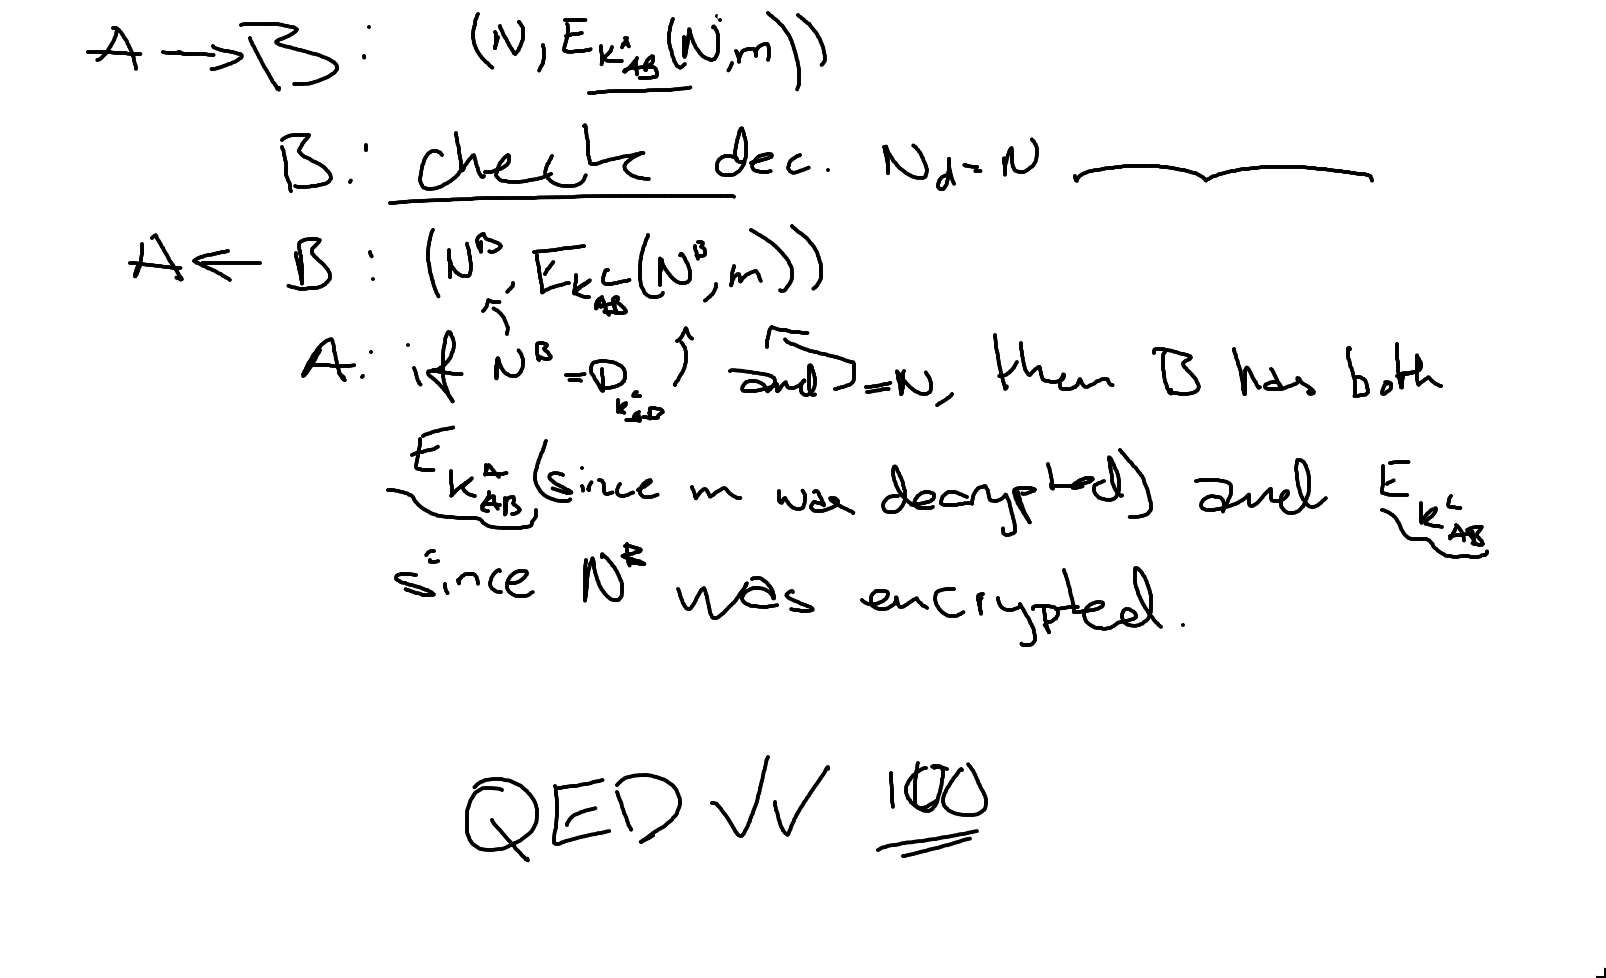
\includegraphics[scale=0.25]{image.png}
% TODO Verify this protocol
\begin{align*}
    \mathcal A &: \mathcal{N} \leftarrow \textsc{RNG}
    \\
    \mathcal{A} &: h \leftarrow \mathbb{H}(\mathcal{N})
    \\
    \mathcal{A} &: m \leftarrow \text{Random string of bytes}
    \\
    \mathcal{A} &: c \leftarrow \mathbb{E}_\mathcal{K_{AB}^{A}}(m, \mathcal{N})
    \\
    \mathcal{A} \rightarrow \mathcal{B} &: (c, h)
    \\
    \mathcal{B} &: (m', \mathcal{N}') \leftarrow \mathbb{D}_\mathcal{K_{AB}^{A}}(c)
    \\
    \mathcal{B} &: \mathbb{H}(\mathcal{N}') = h \implies m' = m
    \\
    \mathcal{B} &: \mathcal{N}_B \leftarrow \textsc{RNG}
    \\
    \mathcal{B} &: c_B = \mathbb{E}_{\mathcal{K_ {AB}^C}}(m, \mathcal{N}_B)
    \\
    \mathcal{B} &: h_B = \mathbb{H}(\mathcal{N}_B)
    \\
    \mathcal{A} \leftarrow \mathcal{B} &: (c_B, h_B)
    \\
    \mathcal{A} &: (m'', \mathcal{N}'') \leftarrow \mathbb{D}_\mathcal{K_{AB}^{C}}(c_B)
    \\
    \mathcal{A} &: m = m'' \land \mathbb{H}(N'') = h_B \implies
    \\
    &\mathcal{B} \text{ knows both } \mathcal{K_{AB}^A} \text{ and } \mathcal{K_{AB}^C}
\end{align*}

\noindent Now we know that $\mathcal{B}$ knows both keys, and as such we can use $\mathcal{K_{AB}^C}$ to encrypt the message and $\mathcal{K_{AB}^A}$ to perform the integrity-verifying hash.

\subsection*{(f)}

One of $\mathcal A$ and $\mathcal B$ decides on a new key. 
It is sent to the other party with a nonce, both encrypted with the already shared key, alongside a hashed version of the nonce, similar to before. That is, $(\mathbb{H}(\mathcal{N}), \mathbb{E}_\mathcal{K_{AB}}(\mathcal{K}_{\textsc{new}}, \mathcal{N}))$.
The receiver checks the hash of the decrypted nonce, and if they match, it sends back the following:
\begin{enumerate}
    \item A new nonce, the received nonce, and the key, all encrypted with the shared key.
    \item The new nonce, hashed.
\end{enumerate}
The sender then checks if the received new hashed nonce matches with the hash of the encrypted one, and also checks that the received key and other nonce matches the ones it sent previously.

\newpage
\section{Asymmetric Key Security Protocols}

\subsection*{(a)}

The first step is the only security issue.
A malicious eavesdropper could tamper with the message and hijack the session completely, impersonating $\mathcal A$ and thus fooling $\mathcal B$. However, this is not too big of an issue, as the only requirement is authenticating $\mathcal{B}$ (which does not depend on this step anyway).
Since the time server is our best chance of security (since it is the only synchronisation we have between the two devices), we will rely on this to authenticate $\mathcal{B}$ by checking that the devices' clocks are almost identical.
This is obviously not secure, especially since the time server is presumably quite in sync with other time servers and computer clocks around the world, but it may be enough if the network latency is low and we are able to have narrow margins because of it.
If, however, the time server can be offset to some random date in time, it becomes more secure as an attacker has to know the date as well, in this case.

\begin{align*}
    \mathcal A \rightarrow \mathcal B &: \mathcal{PK_A}
    \\
    \mathcal{A} \leftarrow \mathcal{B} &: \textsc{Enc}_{\mathcal{PK_A}}([\mathcal{PK_B}, \mathcal T_{\textsc{Clock}}^{\mathcal B}])
    \\
    \mathcal A &: c \leftarrow \textsc{Received}
    \\
    \mathcal A &: [\mathcal{PK_B}', \mathcal{T^B}'] \leftarrow \textsc{Dec}_{\mathcal{K_A}}(c)
    \\
    \mathcal A &: \mathcal{T^B}' \textsc{ reasonably close to } \mathcal{T}_{\textsc{Clock}}^{\mathcal A} \implies 
    \\ &\qquad \mathcal{PK_B}' = \mathcal{PK_B}
\end{align*}

\subsection*{(b)}
As mentioned in (a), we are not entirely secure as neither device has any of the others' keys and thus has to rely on a synchronised clock for security. The extra steps required could be done in two main ways:
\begin{enumerate}
    \item Share $\mathcal{A}$'s public key with $\mathcal{B}$ or vice versa.
    \item Give both devices access to a key server or database, from which they can securely retrieve keys.
\end{enumerate}
There are pros and cons with each solution. The first one is more secure, as the key would already be hard-coded into one of the devices, but would also be cumbersome in the sense that each device has to manually get the key placed onto it. If the first one is to be implemented, the best way to authenticate $\mathcal{B}$ would be to give its public key to $\mathcal{A}$ instead of vice versa as it would require less steps (as we already have $\mathcal{PK_B}$ and know that it corresponds to $\mathcal{B}$), but giving $\mathcal{A}$'s to $\mathcal{B}$ would work too, albeit less efficient (we send a request signed with $\mathcal{K_A}$ to $\mathcal{B}$ who verifies this and replies with $\mathbb{E}_\mathcal{PK_A}(\mathcal{PK_B})$).% and then start encrypting the pings with $\mathbb{D}_\mathcal{K_A}(\mathbb{E}_\mathcal{PK_A}(\mathcal{PK_B})) = \mathcal{PK_B}$).
\\
\\
The second solution, as mentioned, is a lot more flexible as $\mathcal{A}$ could just pull the public key of any device it wishes to authenticate (and ping), but this requires a secure connection to this server as well as that the server itself is secure. If we are able to trust this, option 2 would give us the most flexibility while not being any less secure.

\subsection*{(c)}
Symmetric encryption is more efficient than asymmetric, which is good for things that need to be handled swiftly and/or often (such as pinging). The short idea is to encrypt the symmetric key, e.g. using the other party's public key as well as signing it with your private key. This means that the recipient $B$ can use $A$'s public key to verify authenticity, and its own private key to access the confidential data. Now, we should also hash the shared key and send said hash in plain text alongside the encrypted/signed key. This is done so that the recipient can verify that the key has actually arrived OK, as if we left out the hash and an attacker tampered with the message, the recipient would try to use a gibberish key.% which would result in a successful denial of service attack as the devices would be unable to communicate but still be trying.
%means that for us to get something wrong which still looks right (false positive), the adversary has to hash $K_{AB} = PK_A(K_B(\text{signed + encrypted key}))$ which is not feasible without the knowledge of $K_B$ (i.e. the only entity able to fool $B$ is $B$ itself).
\\
%Non-funky version which is actually understandable: Send $(K_A(PK_B(K_{AB})), \text{SHA-1}(K_{AB}))$. This is authenticated due to sign, and confidential due to encryption. B gets key and can compare it using a known hash, but no-one can reverse the key from the hash nor from the signed/encrypted key.

\begin{align*}
    \mathcal{A} &: c \leftarrow \textsc{Enc}_{\mathcal{PK_B}}(\mathcal{K_{AB}})
    \\
    \mathcal{A} &: \sigma \leftarrow \textsc{Sign}_{\mathcal{K_A}}(c)
    \\
    \mathcal{A} &: h \leftarrow \mathbb{H} (\mathcal{K_{AB}})
    \\
    \mathcal{A} \rightarrow \mathcal{B} &: (\sigma, h)
    \\
    \mathcal{B} &: \text{if } c' \leftarrow \textsc{Ver}_{\mathcal{PK_A}}(\sigma) \text{ succeeds}
    \\
    \mathcal{B} &: \mathcal{K_{AB}}' \leftarrow \textsc{Dec}_\mathcal{K_B}(c')
    \\
    \mathcal{B} &: \mathbb{H}(\mathcal{K_{AB}}') = h \implies \mathcal{K_{AB}}' = \mathcal{K_{AB}}
    \\
    \mathcal{A} \leftarrow \mathcal{B} &: \textsc{Enc}_{\mathcal{K_{AB}}}(\text{"OK"})
\end{align*}

\newpage
\section{Jamming Impact on End-to-end Wireless Communications}
\subsection*{Assumptions, Data and Used Symbols}

Following are the \textbf{assumptions} made:

\begin{enumerate}
    \item In our solutions we assume that each arrow constitutes one path and that the event of any path being jammed is independent of the others.
    \item Furthermore, we assume that paths with different numbers could be used interchangeably, i.e. one can use channel $1$ to get from $A$ to $B$ but channel $2$ to get from $B$ to $C$.
\end{enumerate}
\\
We have the following data:

\begin{itemize}
    \item Probability of any one path being blocked: $p$
    \item Probability that there is no available channel from A to C: $N$
\end{itemize}
\\
Notation used are $XY$, meaning there is a path from $X$ to $Y$.
A specific path is given by $X _i Y$, stating there is a path $i$ from $X$ to $Y$.
Similarly, $\neg XY$ specifies that all paths between $X$ and $Y$ has been jammed.
Further, let $\beta_n$ signify the event that $n$ paths are blocked.

\subsection*{Question 1}

We want to calculate $P(AB \mid \neg AC)$.
We know that $\neg AC \implies \neg AB \lor \neg BC$.
That there is a path $AB$ given $\neg AC$, only has three possible combinations: $A_1B \land A_2B$, $A_1B \land \neg A_2B$ and $\neg A_1B \land A_2B$.
\\
\\
%$P(\neg AC) = P(Three paths blocked) + P(four paths blocked) + P(AB both 1 and 2 blocked OR BC both 1 and 2 blocked)$
%\\
%\\
%so e.g. three paths blocked results in AB only half the time (3 blocked = 1 unblocked) and so we get $0.5 * P(3 blocked) = 0.5 * p^3 * (1-p) $
%and two blocked gives 4 choose 2 = 6 possible outcomes, only one of which results in AB being blocked $\implies$ 1/6 * P(2 blocked)
%% P(AB)=sum( P(n blocked) * P(AB blocked | n blocked) ) for n \in {1,2,3,4}
%\\
%\\
% We define $\beta_n$ as $n$ paths being blocked.
% Bayes theorem: $P(A \mid B) = \frac{P(B \mid A) P(A)}{P(B)}$
% \\
% so we have $P(AB \mid \neg AC) = \frac{P(\neg AC \mid AB) P(AB)}{P(\neg AC)}$
% \begin{itemize}
    % \item $P(AB) = \sum_{n=0}^4 P(\beta_n) P(AB \mid \beta_n) = (1-p)^4 \cdot 1 + p(1-p)^3 \binom{4}{1} \cdot 1 + p^2(1-p)^2 \cdot \binom{4}{2} \cdot \frac{5}{\binom{4}{2}} + p^3 (1-p) \cdot \binom{4}{1} \cdot \frac{2}{\binom{4}{1}} + p^4 \cdot 0$ \\
    % $= (1-p)^4 + p(1-p)^3 + 5 p^2 (1-p)^2 + 2 p^3 (1-p)$
    % \item
        % $P(\neg AC) = P(\beta_3)+P(\beta_4)+P(\beta_2 \land \neg AB) + P(\beta_2 \land \neg BC) = p^3(1-p)\binom{4}{3}+p^4+2p^2(1-p)^2$
    % \item $P(\neg AC \mid AB) = P(\neg BC \mid AB) = P(\beta_2 \land \neg BC) + P(\beta_3 \land \neg BC) = p^2(1-p)^2 + 2p^3(1-p)$
% \end{itemize}
% 
% \\
% \\
Since $\neg AC$ can be split up into several disjoint outcomes: $\beta_2 \land \neg AB$, $\beta_2 \land \neg BC$, $\beta_3$, $\beta_4$, we can write $P(AB \mid \neg AC)$ as a sum of all its cases according to the law of total probability, like so:
\begin{align*}
P(AB \mid \neg AC) &= P( AB \mid \beta _2 \land \neg BC) \cdot P(\beta _2 \land \neg BC) \\
&\qquad+ P(AB \mid \beta_2 \land \neg AB) \cdot P(\beta _2 \land \neg AB) \\
&\qquad+ P(AB \mid \beta_3) \cdot P(\beta _3) \\
&\qquad+ P(AB \mid \beta_4) \cdot P(\beta _4) \\
&= 1 \cdot p^2(1-p)^2 + 0 + \frac{2}{4}p^3(1-p)+0 \\
&=p^2(1-p)^2+\frac{p^3(1-p)}{2}
\end{align*}

\subsection*{Question 2}

We add a path $A_3C$ to the map.
We are still looking for $P(AB \mid \neg AC)$.
Now the set of possible jammings leading to $\neg AC$, where $AB$ is still possible, is different (note that we are ignoring all situations that imply $\neg AB$): $\beta_3 \land \neg AC \land \neg BC$, and $\beta_4  \land \neg AC \land \neg BC$.
The reason why we do this, is that $\neg A_3C$, $\neg BC$ must hold for $\neg AC$ to hold if $AB$ holds.

\begin{align*}
P(AB \mid \neg AC) &= P(AB \mid \beta_3 \land \neg A_3C \land \neg BC) P(\beta_3 \land \neg A_3C \land \neg BC) \\
&\qquad + P(AB \mid \beta_4 \land \neg A_3C \land \neg BC) P(\beta_4 \land \neg A_3C \land \neg BC) \\
&= 1 \cdot p^3(1-p)^2 + 1 \cdot p^4(1-p) \cdot 2 \\
&= p^3(1-p)^2 + 2p^4(1-p)
\end{align*}

\newpage
\section{Channel Jamming}
\subsection*{What is the probability that a packet is lost due to jamming on any transmission?} \\
We're looking for the probability that both the transmitter and the jammer choose the same channel, which is the sum of the probabilities of them both choosing channels 1 through 4 at the same time. 
Since they are independent events, the probability of them occurring at the same time is the product of the probabilities.
Let $T_i$ symbolise that the transmission takes place on channel $i$, and $J_i$ that channel $i$ is being jammed.
\begin{align*}
    \sum _ {i \in \{1,2,3,4\}}P(T_i \land  J_i)  &= \sum _ {i \in \{1,2,3,4\}}P(T_i)P( J_i) \\
    &= P(T_1)P(J_1)+P(T_2)P(J_2)+P(T_3)P(J_3)+P(T_4)P(J_4) \\
    &= 0.1\cdot 0.4 + 0.2\cdot 0.3 + 0.5 \cdot 0.2 + 0.2\cdot 0.1 \\
    &= 0.04+0.06+0.1+0.02 = 0.22
\end{align*}

\subsection*{What is the probability that there will be 5 successful transmissions in a row?} \\
Let $F$ be the event of failed transmission, and $S$ successful transmission. We know that $P(F) = 0.22$, and as transmissions succeeding are independent events we get:
\\
\\
$P(\text{5 in a row}) &= P(S)^5 = P(\neg F)^5 = (1-P(F))^5 = (1-0.22)^5 = 0.78^5\approx 0.29$
% 0.1, 0.2, 0.5, 0.2
% ...maps to ...
% 0.4, 0.3, 0.2, 0.1
% which gives
% 0.04+0.06+0.1+0.02 = 0.22

\newpage
\section{Frequency Hopping Spread Spectrum Anti-jamming}

\subsection*{Question 1}

\subsubsection*{What is the probability that a transmission that lasts 1 second is unjammed?}
The probability of choosing channel $i$, where we can call $C_i$, is $P(C_i)=\frac{1}{10}$.
A transmitter being used for 1 second will select a channel $1/0.2 = 5$ times.
Probability of a successful transmission of 200 ms is $P(\neg J_{i})=\frac{7}{10}$, i.e. the probability of randomly choosing a non-jammed channel.
Doing so five times in a row is done with a probability of $P(\neg J)^5=0.7^5 \approx 0.17$, as ''duplicate'' choices are possible, meaning $P(C_i)$ is the same for all $i$ during the entire process.

\subsubsection*{What is the probability that 40\% of the transmission is jammed?}

40 \% of the transmission means that exactly 2 of the 5 chosen channels were jammed, which has a probability of $0.7^3+0.3^2 \approx 0.03$. There are $\binom{5}{2}=10$ combinations of this situation, and thus the probability is $P(\text{40\% success-rate})=0.7^3 \cdot 0.3^2\cdot \binom{5}{2} \approx 0.31$.
This holds by the law of total probability.

\subsection*{Question 2}

\subsubsection*{(a)}

For each 200 ms interval, if the channel has been detected as blocked, exclude this from the list to pick the next channel from.
We would then get blocked three transmissions at most and would definitely succeed with two, since the jammer only jams three fixed channels. To give an example, this means that the first channel we try has a 30\% risk of failure (being jammed), but if this first channel is jammed, the second channel no longer has a 30\% risk but instead a $\frac{2}{9} \approx 0.22 \implies$ 22\% risk (and after two jammed channels, P(third jammed) = $\frac{1}{8}$ for the same reasons).

\subsubsection*{(b)}

In the long run (i.e. an infinitely long transmission) it doesn't matter how many channels are jammed -- as long as there is one available channel transmission success-rate would steadily increase and approach the limit of 100\%.
\\
\\
The main point is that we get a lower risk of failure in the long run and thus have increased the reliability of communication. Of course, this all relies on the fact that the jammer does not change channels.

\subsubsection*{(c)}

If the transmitter stops choosing pseudo-randomly after realising that a channel is unjammed, the probability of a one-second transmission being unjammed is 0.7 (since only the first channel matters - if this is unjammed, we continue there and thus don't get jammed at all, but if it \textit{is} jammed, we no longer have an unjammed transmission. Also, this means that the event of being 40\% jammed can only occur by choosing $J, J, U$ ($J$ being jammed and $U$ being unjammed), which gives the probability $\frac{3}{10} \frac{2}{9} \frac{7}{8} = \frac{42}{720} = \frac{7}{120}$.
\\
\\
If the jammer chooses different channels each time, there is no way to predict and minimise failure by the transmitter.
However, this only holds if the jammer chooses channels in a uniformly distributed manner; otherwise, the transmitter could (theoretically) use machine learning or other probabilistic methods to learn the behaviour of the jammer and in that way minimise failed transmissions.

\newpage
\section{Flooding}

\subsection*{Statement 1 -- buffer}
Allocating less resources for network A means that we may negatively affect a \textit{large number} of legitimate hosts based upon the fact that there are \textit{some} bots on the same network.
%Punishing all machines on a network based on a few malicious users is like punishing a whole society for a single criminal's wrongdoings.
Therefore, it would make more sense to allocate any leftover space (not needed to serve network B) as extra buffers for network A, since the smaller our network A-buffer is, the easier it will be for the bots to succeed in their DDoS attack. %Assuming our non-ACK:ed SYN requests get dropped after a certain time $\tau$, the only thing that happens when we increase the buffer size for network A is that it gets harder to succeed with a (D)DoS attack -- there are no negative consequences to it whatsoever (as long as it does not infringe on the network B buffer).


\subsection*{Statement 2 -- firewall}

In a similar fashion, but even harsher, this punishes a large number of legitimate users based on a few malicious ones.
This is worse than the first statement as one completely cut connections from network A.
Another problematic aspect of this solution is that malicious bots could most likely spoof their IP addresses and thus bypass the firewall anyway, making the legitimate users the only ones with denied access.

\subsection*{Statement 3 -- SYN-block}

This basically disables establishing new connections to from network A, which is a bad idea.
Though, this is an efficient way to block traffic, alas it might be too efficient.
The only time this is reasonable, is if serious malware is being shared through the bots on network A, but given that this knowledge is shared, it might already be too late to counter infection with such SYN-blocking.

\subsection*{Statement 4 -- packet marking}

This is something that \textit{could} be useful as it gives more data on how the packets have travelled, but it depends on how it is implemented. A good solution would be one where marking is only done on important routers (i.e. A, B, C, D, E, F; all packets only have one way through G and H anyway), and where routers only add markings if there is available space in order to not overwrite existing marks.
This will ensure that we can always view the order of the starting routers, and spoofing IPs is as a result not as efficient: if we spoof our IP to be something outside of network A, we can see that it is spoofed thanks to the routers' markings, and as such drop it. This means that we can only reliably spoof our IPs to be one within network A, and as such not evade any restrictions imposed on such IPs.
%If the goal is to block communication from network A, this is an inefficient solution, yet secure to guarantee packet's actual source address.
\\
\\
However, this solution would not directly help with bots sending packets with a spoofed IP coming from within network A. As such, the best overall solution would most likely be a combination of this (to limit IP spoofing) and perhaps a larger buffer for network A (to handle the malicious requests easier).
\\
\\
Of course, all of this relies on the assumption that we can design the packet marking protocol ourselves (hinted at in the assignment where router D can \textit{decide} to mark a packet). If all routers always mark the packet and we only have three available spaces for markings, this method is completely useless -- we will always end up with (F, G, H) regardless of whether the packet came from network A or network B.

\newpage
\section{Distributed Denial of Service}

\subsection*{(a)}
That would be all hosts in the aforementioned networks, i.e. $2^7+2^9+2^{10}=1664$ hosts in total.
Each specified IP-range gives us $2^{32-m}$ addresses, where $m$ is the subnet mask.

\subsection*{(b)}
We know that each new connection adds one TCB entry to the server's memory; the size of the SYN segment is not relevant here, as it is only used to initiate the connection and is not stored. Assuming ''Gbytes'' refers to ''Gibibytes''/GiB which is $2^{30}$ bytes, we need $\lceil \frac{2^{30}}{192} \rceil = \lceil \frac{2^{30}}{2^7 \cdot 1.5} \rceil = \lceil \frac{2^{23}}{1.5} \rceil = 5592406$ connections (or SYN-segments) to exhaust the server's memory. \\
Note: If ''Gbytes'' refers to a Gigabyte, or GB, we just perform the calculation with $10^9$ bytes instead of $2^{30}$, giving us $\lceil \frac{10^9}{192} \rceil = 5208334$ SYN-segments.

\subsection*{(c)}

Each host could send $2\cdot 10^6$ bits per second, i.e. $250$ KB/s.
Assuming that we have 1 GB as in $10^9$ B in the server connection table, it would then take $\frac{10^9}{0.25\cdot 10^6}=4\cdot 10^3$ seconds to flood the web server by a single attacker, given that there is no timeout on the connections.
This corresponds to roughly 1 hour and 7 minutes, and assumes that the attacker can generate packets fast enough to saturate their network bandwidth.

\subsection*{(d)}

Given that all hosts attack at the same time, the total bandwidth being sent is $0.25 \cdot 1664=416$ MB/s.
However, this surpasses the capacity of 3 Gb/s (= 375 MB/s) of the bandwidth of the symmetric link.
Thus, the maximum workload sent to the server would be limited by the link's bandwidth.
As a result, the web server's link would be flooded/congested as soon as the attackers' packets reach it.
Furthermore, exhausting the memory would then take $\frac{10^9}{0.375\cdot 10 ^9}\approx 2.67$ seconds.

\subsection*{(e)}

As exhaustion occurs after $2.67$ seconds of maximum bandwidth use, the threshold of discarding connections must be lower than so to decrease flooding of memory. This also means that the number of attackers is less relevant, as their capabilities are limited by the bandwidth.
Moreover, the congestion of the link is nothing that the web server really could do anything about, and and so a good choice of $\tau$ could be anything $\leq 2.5$ seconds. % (but preferably something like $2$, just to have a bigger margin while still allowing for slower connections/communication).
If $\tau$ is chosen too low, possibly $\leq 1$, a flooding attack on the link %(i.e. as a result of another attack)
would increase the risk of failed connections by a lot.
When the bandwidth of the link is congested, the risk of losing TCP packets increases which would negatively affect legitimate users.
%We do not want to set $\tau$ to anything too low, either, as this could negatively affect legitimate users that may not be able to send their ACK in time during an attack.
\newpage
\section{Password Management}

\subsection*{(a)}

We have $\mathcal{H}=\mathcal{L}\cdot \log_2 \mathcal{N} = 8\log_2 256 = 8 \cdot 8 = 64$.

\subsection*{(b)}

No, it does not.
Entropy only depends on the length and alphabet size.
Frequently changing passwords to the same length and having the same restriction of characters would therefore maintain the same entropy.

\subsection*{(c)}

The amount of combinations when the password has a length of 10 is $256^{10}=(2^8)^{10}=2^{80}$.
If the attacker could try $2\cdot 10^{7}$ combinations per second, the time it would take would be limited by $\frac{2^{80}}{2 \cdot 10^7}\approx 6.04 \cdot 10^{16}$ seconds.
This equals to approximately 1.9 billion years.
\\
\\
As each password is random, the probability of each combination is equally probable.
Given one specific hash, the expected time would therefore be the half of the previous question, i.e. roughly 950 million years.

\subsection*{(d)}

If a password is hashed with a non-leaked salt, as it is in this case, it does not matter if the KDF is leaked.
A dictionary attack could then not be effective, as the salt would be needed to be guessed as well which increases the time substantially.

\subsection*{(e)}

Assuming the salt is not leaked and we conduct the brute force by guessing a password, applying the salt and then hashing the result (rather than just attempting to find collisions), it would increase the complexity by a factor of $2^{128}$ as this is the amount of combinations per password we would have to try.
If the salt \textit{is} leaked, however, the only added complexity is that we need to perform the hashing algorithm on the password ourselves before checking if it matches -- in other words, we can no longer use rainbow tables.

\subsection*{(f)}

No, it is not, as the password and the generated key have the exact same entropy. The only strength that could be gained such a transformation is if the original password was in any way more predictable than the derived key, which it is not in this case due to being random.

\subsection*{(g)}

There is a major problem, yes. The loop is effectively a \verb|nop|, as it doesn't actually run the password through the hashing algorithm. Instead, it runs a supposed ''hash'' (which is just a random word and not the hashed password) through the algorithm, and this ''hash'' is not used in the final key at all. That piece of code is the same as just doing \verb#key = SHA2(salt||password);# once.

\subsection*{(h)}
This really ought to be a function taking the password, number of iterations and salt as parameters, but to keep it as close to the original code as possible we'll just alter that:

\begin{verbatim}
password = ”Mypw123zxc”;
iterations = 390000; # Defualt value for PBKDF2 in pyca
salt; # Assume randomly generated 32 hex digits
password = SHA2(salt||password);
for(i = 0; i < iterations; i++){password = SHA2(password)};
\end{verbatim}

% \begin{verbatim}
% password = input()
% 
% for _ in range 10:
    % time.sleep(random.int(10, 50), "milliseconds")
% salt = random.hex_string()
% 
% for _ in range 10:
    % time.sleep(random.int(10, 50), "milliseconds")
    % 
% key = SHA2(password, salt)
% \end{verbatim}





\newpage
\section{Firewalls}
We use ''EST.'' in place of ''ESTABLISHED'' here to avoid an unnecessarily wide table.

\begin{table}[h!]
\begin{adjustwidth}{-1.5in}{-1.5in}
    \centering
    \begin{tabular}{c|c|c|c|c|c|c|c}
         Direction & Source & Dest. & Protocol & Src port & Dest. port & State & Action \\
         \hline
         \hline
         IN & * & 17.0.0.0/8 & UDP & * & * &  & DROP \\
         OUT & * & 17.0.0.0/8 & UDP & * & * &  & DROP \\
         IN & 207.46.130.0/24 & 17.0.0.0/8 & * & * & * & NEW,EST. & DROP \\
         OUT & * & 69.171.239.12 & TCP & * & 443 & NEW,EST. & ACCEPT \\ % Facebook
         OUT & * & 69.171.239.12 & TCP & * & 80 & NEW,EST. & REJECT \\ % Facebook
         IN & 64.233.160.0/24 & 17.0.0.1 & TCP & * & 80 & NEW,EST. & ACCEPT \\
         % The ICMP rule below is redundant as it will be dropped at the end anyways
         %IN & * & 17.0.0.0/8 & ICMP & & & & DROP \\
         IN & 64.233.160.0/24 & 17.0.0.0/8 & TCP & * & 22 & NEW,EST. & ACCEPT \\
         OUT & 17.0.0.0/8 & * & TCP & * & 22 & NEW & REJECT \\
         OUT & 17.0.0.0/8 & * & TCP & * & 53 & NEW,EST. & ACCEPT \\
         OUT & 17.0.0.0/8 & * & UDP & * & 53 &  & ACCEPT \\
         IN & * & * & * & * & * & NEW,EST. & DROP \\
         OUT & * & * & * & * & * & NEW,EST. & DROP
    \end{tabular}
    \caption{Firewall rules}
    \label{tab:firewall_rules}
    \end{adjustwidth}
\end{table}

\end{document}